%----------------------------------------------------------------------------------------
%	SOLUTION 2
%----------------------------------------------------------------------------------------
\subsection*{Solution 2.a}
Error rates for different k in k-nearest neighbor algorithm on Optdigit dataset have been tabulated in the table below:
\begin{table}[h!]
	\begin{center}
		\begin{tabular}{||c | c | c | c | c ||} 
			\hline
			k & 1 & 3 & 5 & 7 \\ [0.5ex] 
			\hline\hline
			Error rate(\%) & 5.387 & 4.040 & 4.377 & 5.387 \\ [1ex]
			\hline
		\end{tabular}
	\end{center}
	\caption{Q2.a: Error-rate Vs. k table}
\end{table}
\subsection*{Solution 2.b}
We performed PCA on Optdigits training data and found the following proportion of variance plot:
\begin{figure}[h!]
	\centering
	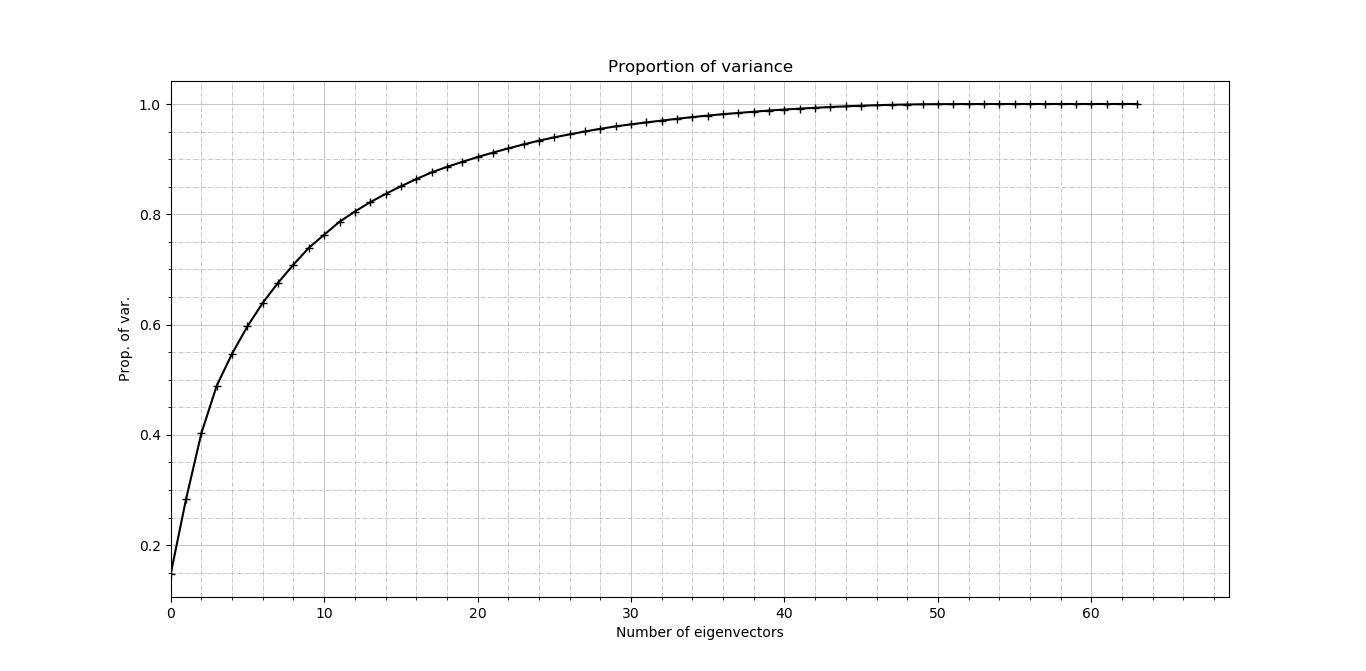
\includegraphics[scale=0.5]{pov_2b}
	\caption{Proportion of variance plot for Optdigits training data}
	\label{fig:pov_2b}
\end{figure}
\newline
We can see from Fig.\ref{fig:pov_2b} that the minimum number of eigenvectors that explain at least 90\% of the variance is 20.
\newline
Therefore, we used 20 principal components for PCA and reduced the dimension of the original Optdigits data to 20. Then, we used KNN on this reduced dimension Optdigits test data. The following table shows the error rates for different k in k-nearest neighbor algorithm on reduced Optdigits test data.
\begin{table}[h!]
	\begin{center}
		\begin{tabular}{||c | c | c | c | c ||} 
			\hline
			k & 1 & 3 & 5 & 7 \\ [0.5ex] 
			\hline\hline
			Error rate(\%) & 4.040 & 4.040 & 4.040 & 4.377 \\ [1ex]
			\hline
		\end{tabular}
	\end{center}
	\caption{Q2.b: Error-rate Vs. k table}
\end{table}
\subsection*{Solution 2.c}
Fig.\ref{fig:optdigits_pca} shows the both Optdigits training and test data after PCA with 2 components.
\begin{figure}[h!]
	\centering
	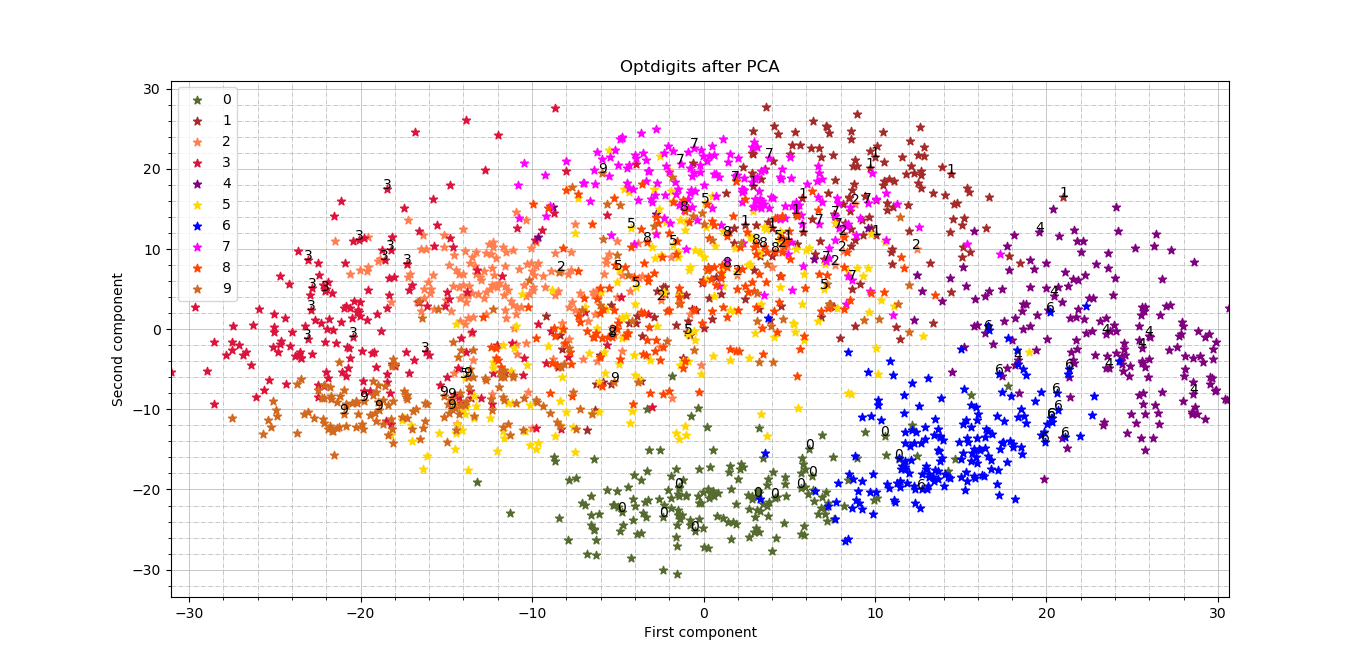
\includegraphics[scale=0.5]{optdigits_pca}
	\caption{Optdigits data after PCA}
	\label{fig:optdigits_pca}
\end{figure}
\subsection*{Solution 2.d}
Table \ref{tbl:l_k_error_2d} shows error rates for different L dimensions and different k neighbors for KNN algorithm on Optdigits test data.
\begin{table}[!h]
\begin{center}
	\begin{tabular}{||c | c | c | c||} 
		\hline
		L & 2 & 4 & 9 \\ [0.5ex] 
		\hline\hline
		k=1 & 44.781\% & 19.191\% &9.764\% \\
		\hline
		k=3 & 41.414\% &18.518\% & 9.427\% \\
		\hline
		k=5 & 40.740\% & 15.824\% & 9.427\% \\ [1ex]
		\hline
	\end{tabular}
\caption{Q2.d: Error-rates for different L dimensions and k neighbors}
\label{tbl:l_k_error_2d}
\end{center}
\end{table}
\subsection*{Solution 2.e}
Fig.\ref{fig:optdigits_lda} shows the both Optdigits training and test data after LDA with 2 components.
\newpage
\begin{figure}[h!]
	\centering
	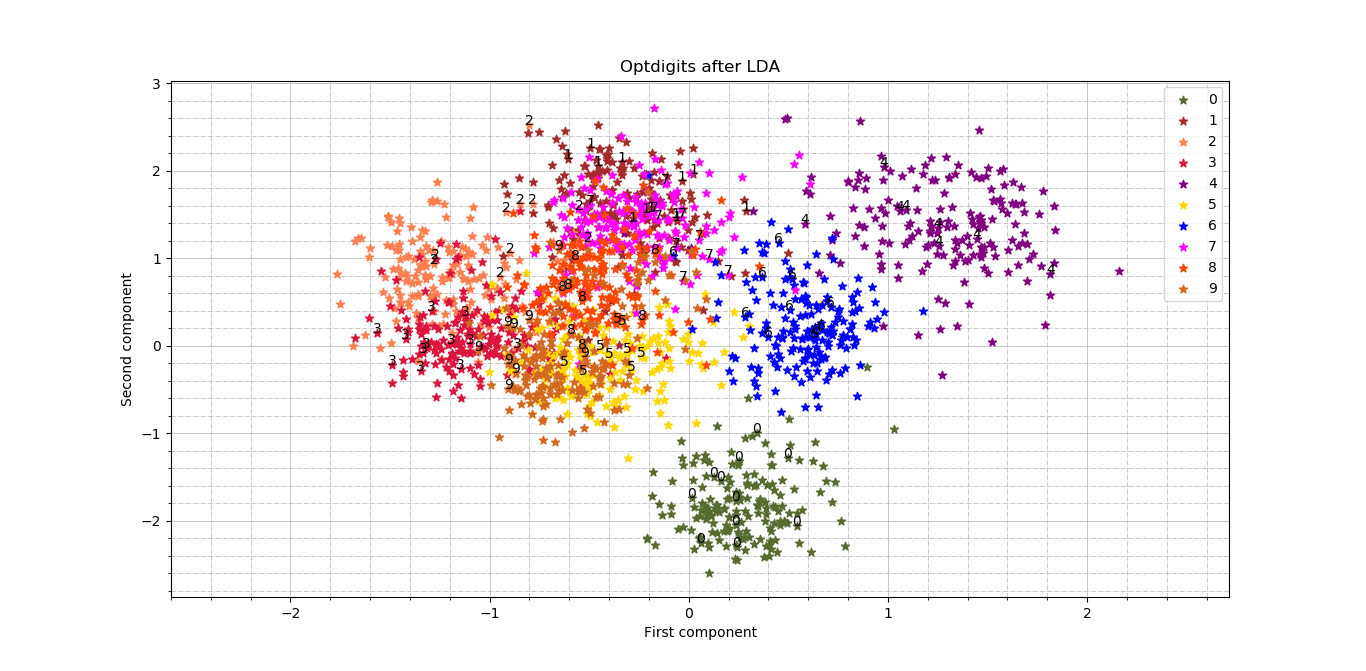
\includegraphics[scale=0.5]{optdigits_lda}
	\caption{Optdigits data after LDA}
	\label{fig:optdigits_lda}
\end{figure}